\documentclass[twocolumn,a4j]{jsarticle}
\setlength{\topmargin}{-20.4cm}
\setlength{\oddsidemargin}{-10.4mm}
\setlength{\evensidemargin}{-10.4mm}
\setlength{\textwidth}{18cm}
\setlength{\textheight}{26cm}

\usepackage[top=15truemm,bottom=20truemm,left=15truemm,right=15truemm]{geometry}
\usepackage[latin1]{inputenc}
\usepackage{amsmath}
\usepackage{amsfonts}
\usepackage{amssymb}
\usepackage[dvipdfmx]{graphicx}
\usepackage[dvipdfmx]{color}
\usepackage{listings}
\usepackage{listings,jvlisting}
\usepackage{geometry}
\usepackage{framed}
\usepackage{color}
\usepackage[dvipdfmx]{hyperref}
\usepackage{ascmac}
\usepackage{enumerate}
\usepackage{tabularx}
\usepackage{cancel}
\usepackage{scalefnt}
\usepackage{multicol}

\renewcommand{\figurename}{Fig.}
\renewcommand{\tablename}{Table }

\lstset{
basicstyle={\ttfamily},
identifierstyle={\small},
commentstyle={\smallitshape},
keywordstyle={\small\bfseries},
ndkeywordstyle={\small},
stringstyle={\small\ttfamily},
frame={tb},
breaklines=true,
columns=[l]{fullflexible},
xrightmargin=0zw,
xleftmargin=3zw,
numberstyle={\scriptsize},
stepnumber=1,
numbersep=1zw,
lineskip=-0.5ex
}

\makeatletter
\newenvironment{table_here}{\def\@captype{table}}{}
\newenvironment{figure_here}{\def\@captype{figure}}{}

\def\@maketitle
{
\begin{center}
{\LARGE \@title \par}
\end{center}
\begin{flushright}
{\large 報告書 NO.09 - 2\quad\@date\quad\@author}
\end{flushright}
\par\vskip 1.5em
}
\makeatother

\setcounter{tocdepth}{3}

\author{来代 勝胤}
\title{令和3年度 1月 第3週 報告書}
\date{2022/1/20}

\begin{document}
\columnseprule=0.1mm

\maketitle
\section*{報告内容}
\begin{enumerate}[1.]
    \item 進捗状況
    \item 二次補間による補正
    \item 卒業論文について
    \item 使用する図表
\end{enumerate}

\section{進捗状況}
今週は卒業論文の執筆と,ラグランジュ補間を用いて不等間隔のデータの処理を行った.

\section{作用力測定装置と校正実験装置の関係}
作用力測定装置から得た抗力方向および揚力方向における出力電圧$V_D$,$V_L$を
正規座標系の$x$軸方向および$y$軸方向の荷重$F_x$,$F_y$に換算する際に,
出力電圧$V_D$,$V_L$と$F_x$,$F_y$の関係性を明らかにするための校正実験を
行う必要がある.
校正実験によって得られた結果を用いて関係性を明らかにするための校正理論について述べる.\\

\subsection{作用力測定装置と校正実験装置の関係}
作用力測定装置と校正実験装置の設置位置によって校正実験結果は大きく変動するため,
その影響を考慮し,補正処理を行う必要がある.
このとき以下のような要因が,校正実験結果への影響を与えていると考えられる.

\begin{enumerate}[(1)]
    \item 作用力測定装置にひずみセンサが正確に取り付けることが難しい
    \item 作用力測定装置が回流水槽に正確に設置することが難しい
    \item 作用力測定装置と校正装置の回転軸を一致させることが難しい
\end{enumerate}

\begin{figure}[htbp]
    \footnotesize
    \begin{center}
        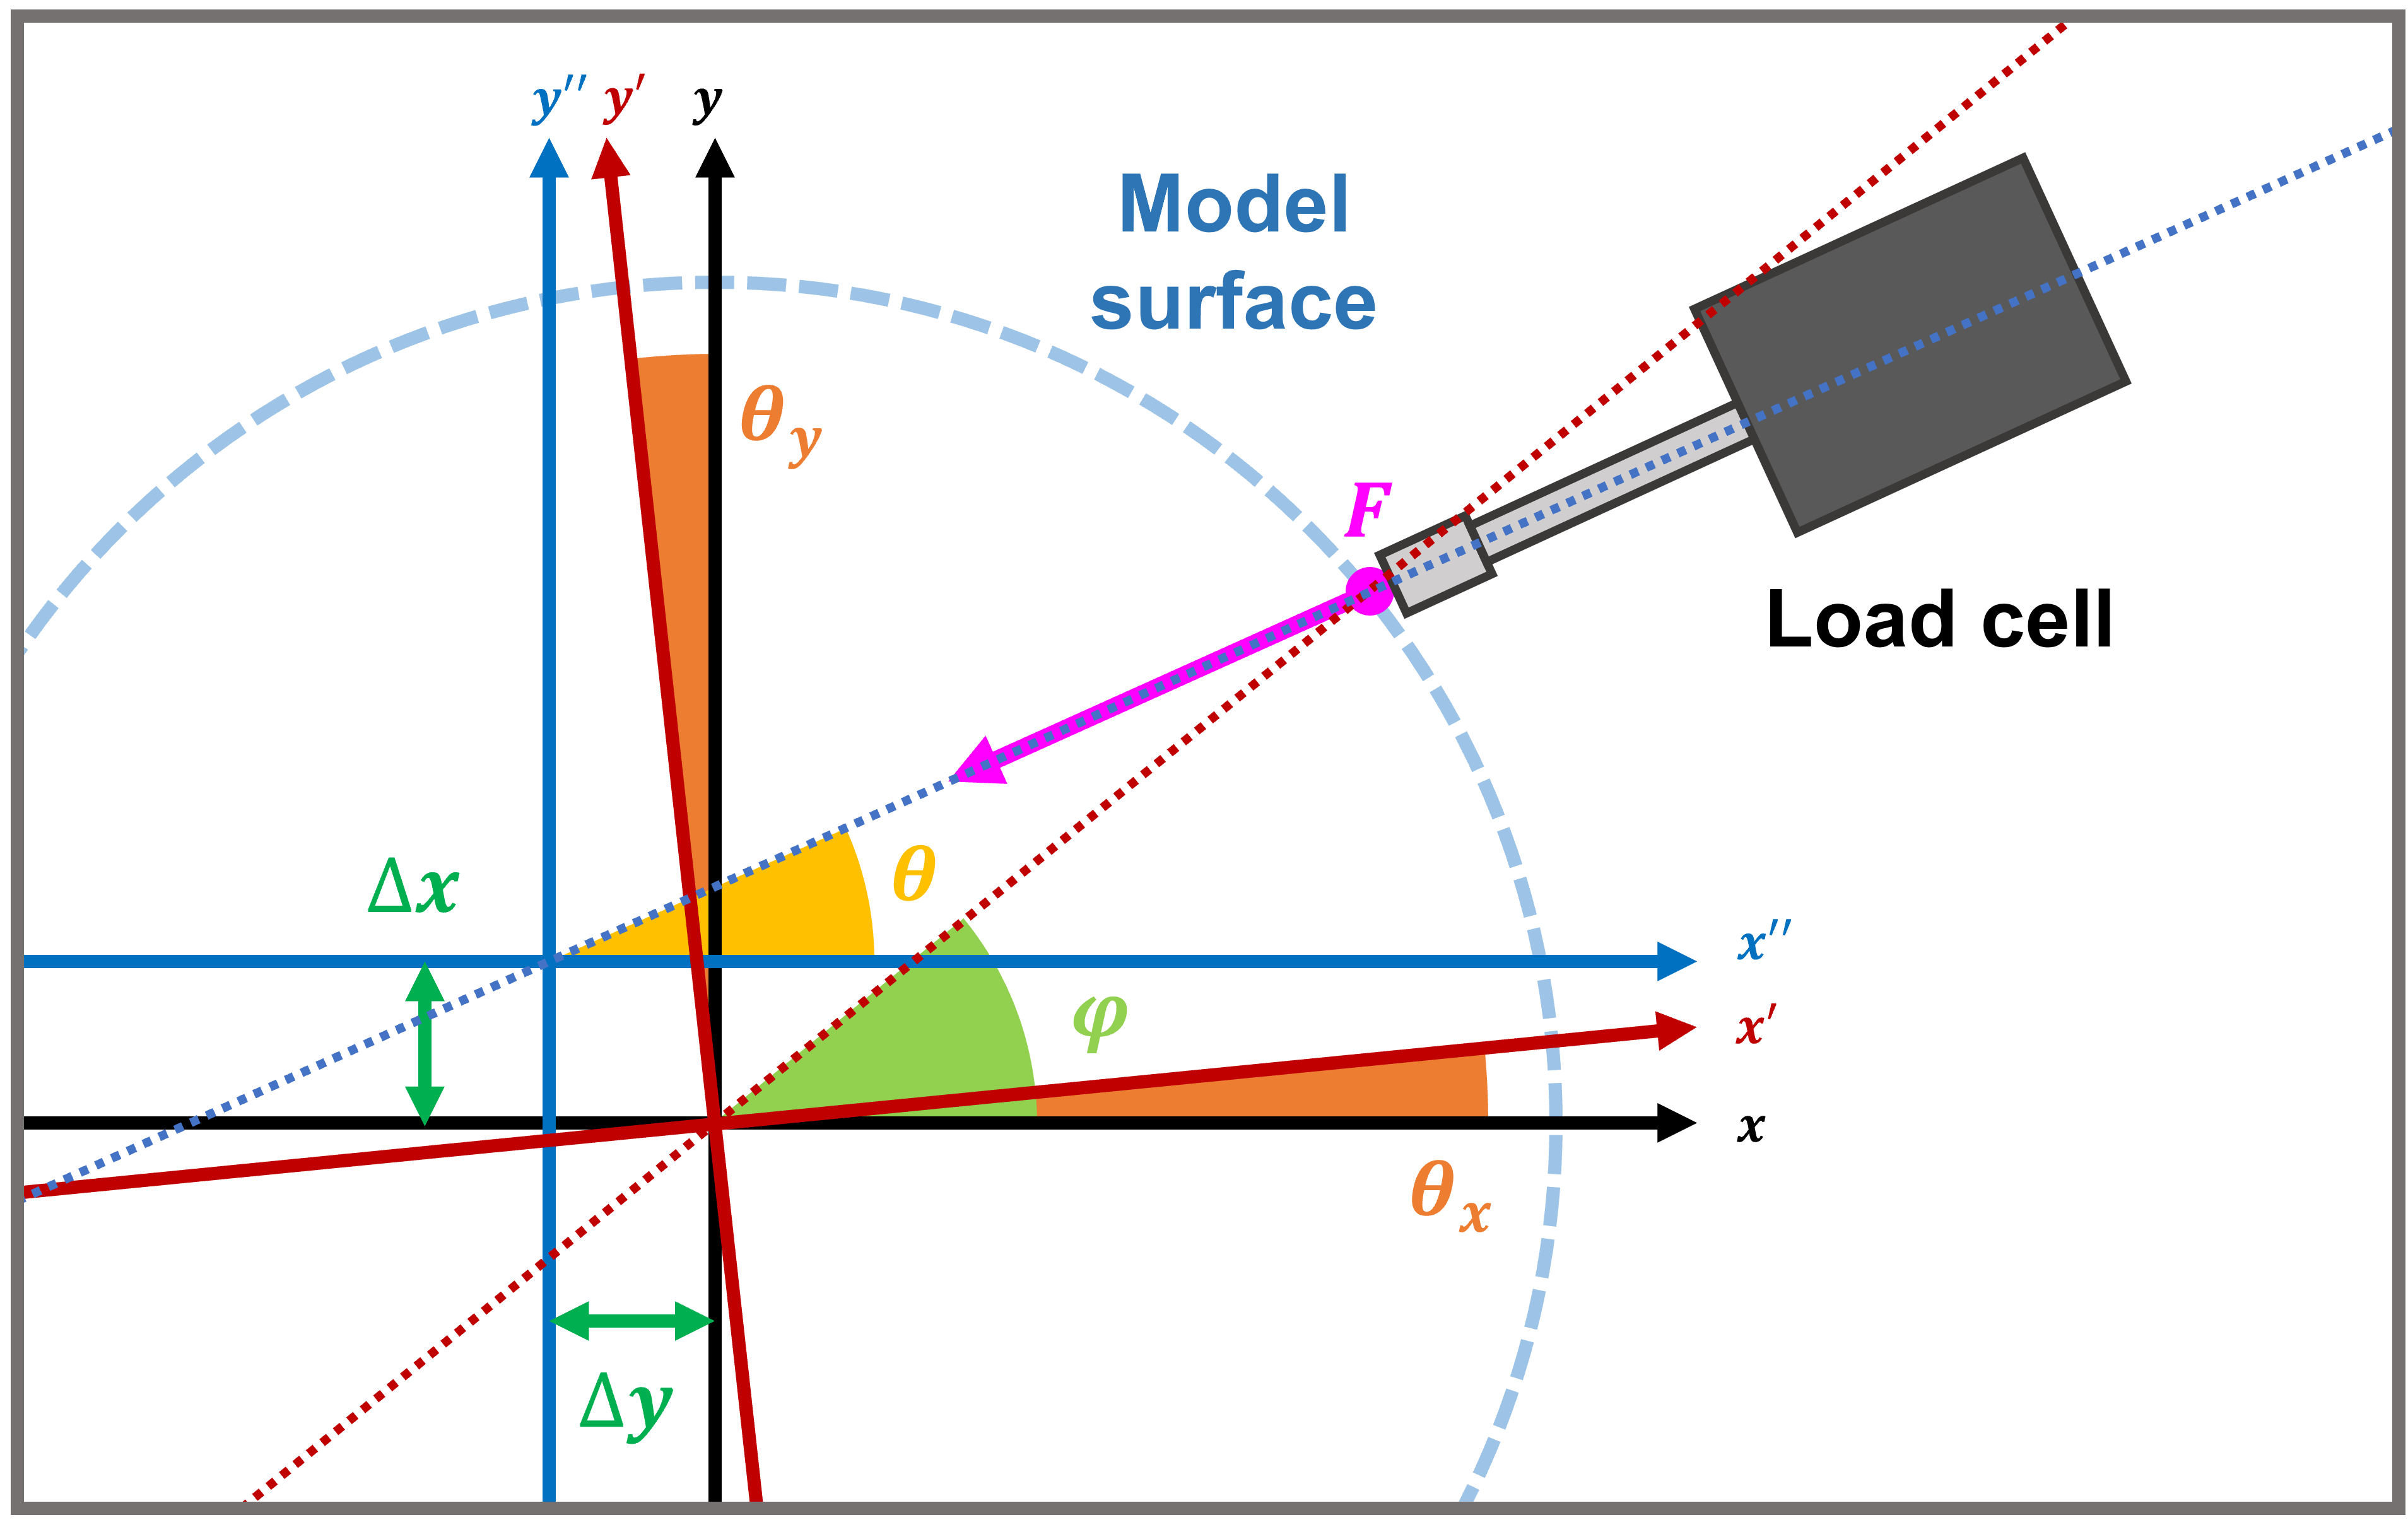
\includegraphics[width=80mm]{../../graduation_thesis/images/31-1.png}
        \caption{}
    \end{center}
\end{figure}

ここで,水流に対する座標系を正規座標系 $(x,y)$,
作用力測定装置の座標系を座標系[1] $(x',y')$,
校正装置の座標系を座標系[2] $(x,'' y'')$とする.

このとき,(1) 作用力測定装置にひずみセンサを正確に取り付けることが難しいこと,
(2) 作用力測定装置が回流水槽に正確に設置することが難しいことから,
座標系[1]は正規座標系に対して
$x'$軸は$x$軸から$\theta_x$,$y'$軸は$y$軸から$\theta_y$だけ回転している.
また,座標系[2]は正規座標系に対して
$x''$軸は$x$軸から$y$方向に$\Delta x$,
$y''$軸は$y$軸から$x$方向に$\Delta y$だけオフセットを持つ状態となる.

\section{二次補間による補正}

\subsection{複合状態における補正理論}

実際に校正実験を行う際には,座標系の回転,オフセットは同時に発生する.
したがって,上記の2つの補正理論を組み合わせて補正処理を行う必要がある.\\

\subsubsection{補正理論の適用順序}

作成した補正理論について,座標系の回転角$\theta_1$,$\theta_2$の特定の際に
離散フーリエ変換を適用することから,座標系のオフセットにおける補正理論を先に適用する必要がある.
また,オフセットを考慮した場合,データ間隔が不等間隔となるため
回転角を特定するための離散フーリエ変換が適用できない.
したがって,ラグランジュ補間を用いて二次近似を行い,等間隔のデータを補完することとした.\\

\subsubsection{ラグランジュ補間}

ラグランジュ補間とは,一般的に以下のように表される.

\begin{align*}
    P\left(x\right)    & = \sum^{n+1}_{i=1} y_i \frac{f_i\left(x\right)}{f_i \left(x_i\right)} \\
    f_i \left(x\right) & = \prod_{k \neq i} \left(x - x_k\right)
\end{align*}
\vskip \baselineskip

ここで,2次補間を行う場合,使用する3点を適切に選択する必要があるが
アルゴリズムを用いて処理を行いたい.
そこで,以下のような手順で補間に使用するデータの選択を行った.

\newpage

\subsubsection{使用するデータの選択}

校正実験では,15度ずつ測定しているため,計24点のデータを得ることができる.
座標系のオフセットにおける補正理論を用いた補正処理では,正規座標系における作用力とその角度が算出される.
しかし,離散フーリエ変換を適用するとき,等間隔のデータが必要となるため15度ごとの補間値を算出しなければならない.
ここで,必要な補間値の角度を$\theta$とするとき,
実際の作用力の角度$\varphi$との差
$\delta \theta$を絶対値で評価することで,その値$|\delta \theta|$が
最も小さくなる角度$\varphi$とその前後のデータを使用することで,$\theta$に最も近い3点を選択することができる.

\begin{align*}
    \delta \theta = |\theta - \varphi|
\end{align*}
\vskip \baselineskip

\subsubsection{テストデータへの適用}
上述の補正理論より座標系の回転・オフセットを考慮したテストデータを作成する.
任意の回転角$\theta_{1\;\mathrm{test}}$,$\theta_{2\; \mathrm{test}}$,
任意のオフセット$\Delta x_\mathrm{test}$,$\Delta y_\mathrm{test}$を与え,
複合状態における出力電圧勾配について,$x''$軸方向を$v_{x''\;\mathrm{test}}$,
$y''$軸方向を$v_{y''\;\mathrm{test}}$とするとき,以下のように表される.

\begin{align*}
    \theta                  & = \frac{\pi}{180} \; i \;\left(i = 0, 1, 2, 3, \cdots\right)                                                       \\
    \alpha                  & = \sin^{-1} \left( \frac{\Delta x_\mathrm{test} \sin \theta - \Delta y_\mathrm{test} \cos \theta}{r} \right)       \\
    \varphi                 & = \theta - \sin^{-1}\left(\frac{\Delta x_\mathrm{test} \sin \theta - \Delta y_\mathrm{test} \cos \theta}{r}\right) \\
    v_{x'' \;\mathrm{test}} & = - \cos \alpha \cos \left(\varphi - \theta_{1\; \mathrm{test}} \right)                                            \\
    v_{y'' \;\mathrm{test}} & = - \cos \alpha \sin \left(\varphi - \theta_{2\; \mathrm{test}}\right)
\end{align*}
\vskip \baselineskip

また,今回を以下のTable 1 のようなパラメータを用いた.

\begin{table}[htbp]
    \begin{center}
        \caption{Test data conditions}
        \begin{tabular}{|p{20mm}|p{20mm}|p{20mm}|p{20mm}|}
            \hline
            \multicolumn{1}{|c|}{$\theta_{1\;\mathrm{test}}$ [deg]} & \multicolumn{1}{|c|}{$\theta_{2\;\mathrm{test}}$ [deg]} & \multicolumn{1}{|c|}{$\Delta x_\mathrm{test}$ [mm]} & \multicolumn{1}{|c|}{$\Delta y_\mathrm{test}$ [mm]} \\ \hline
            \multicolumn{1}{|c|}{10.0}                              & \multicolumn{1}{|c|}{-5.0}                              & \multicolumn{1}{|c|}{5.00}                          & \multicolumn{1}{|c|}{-2.50}                         \\ \hline
        \end{tabular}
    \end{center}
\end{table}

Case 7 に対する座標系の回転おける補正理論の適用過程について説明する.
はじめに,作成したテストデータを以下のFig.2に示す.

\begin{figure}[htbp]
    \footnotesize
    \begin{center}
        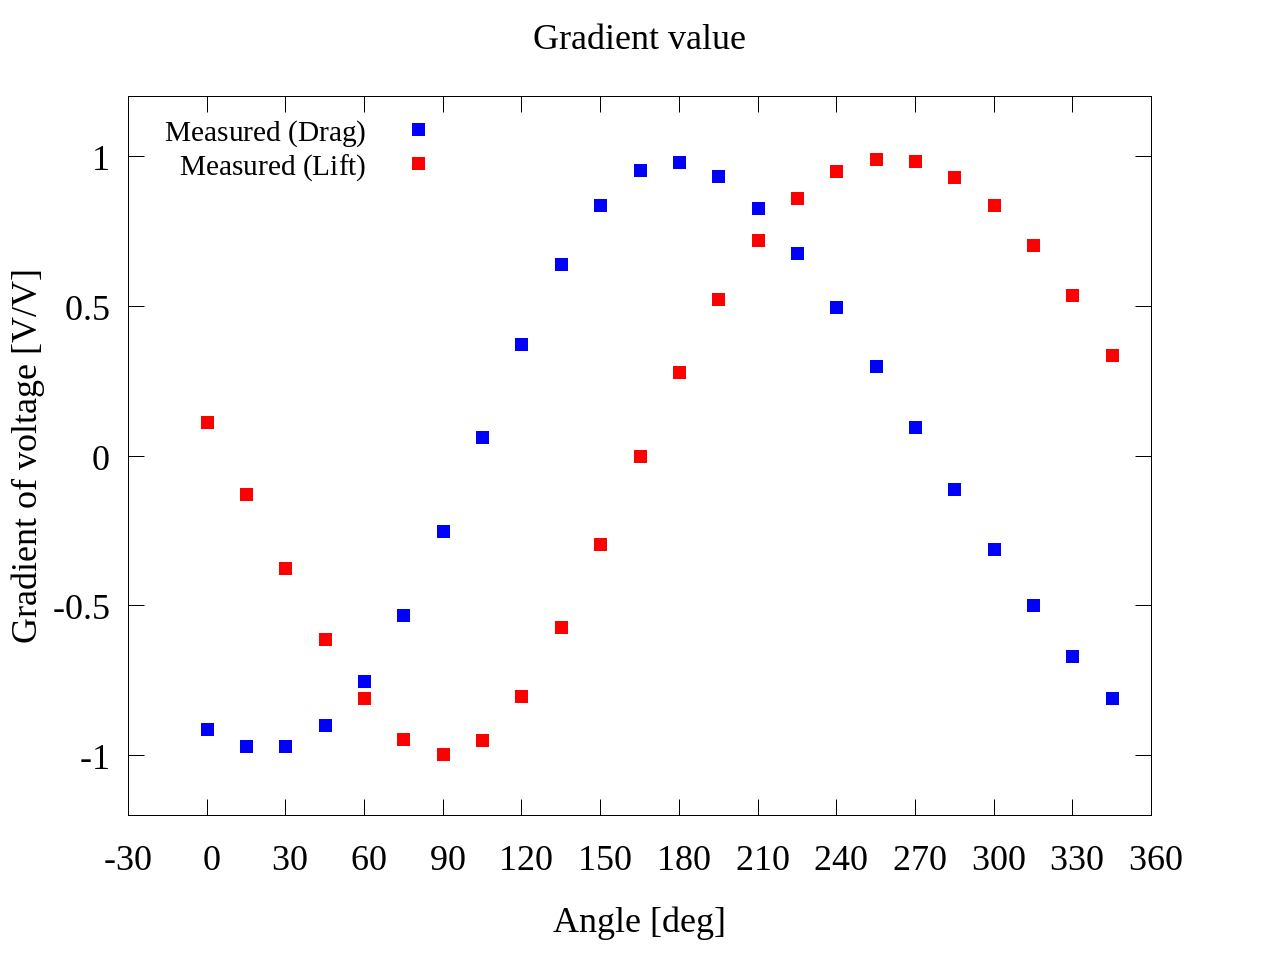
\includegraphics[width=85mm]{../../../02_workspace/result/simulation_tx=10.0_ty=-5.0_dx=5.00_dy=-2.50/plot/05/05_summary-wave.png}
        \caption{Simulated data }
    \end{center}
\end{figure}

\newpage

ここで,座標系のオフセットにおける補正理論を適用した結果を以下のFig.3,Fig.4に示す.

\begin{figure}
    \begin{center}
        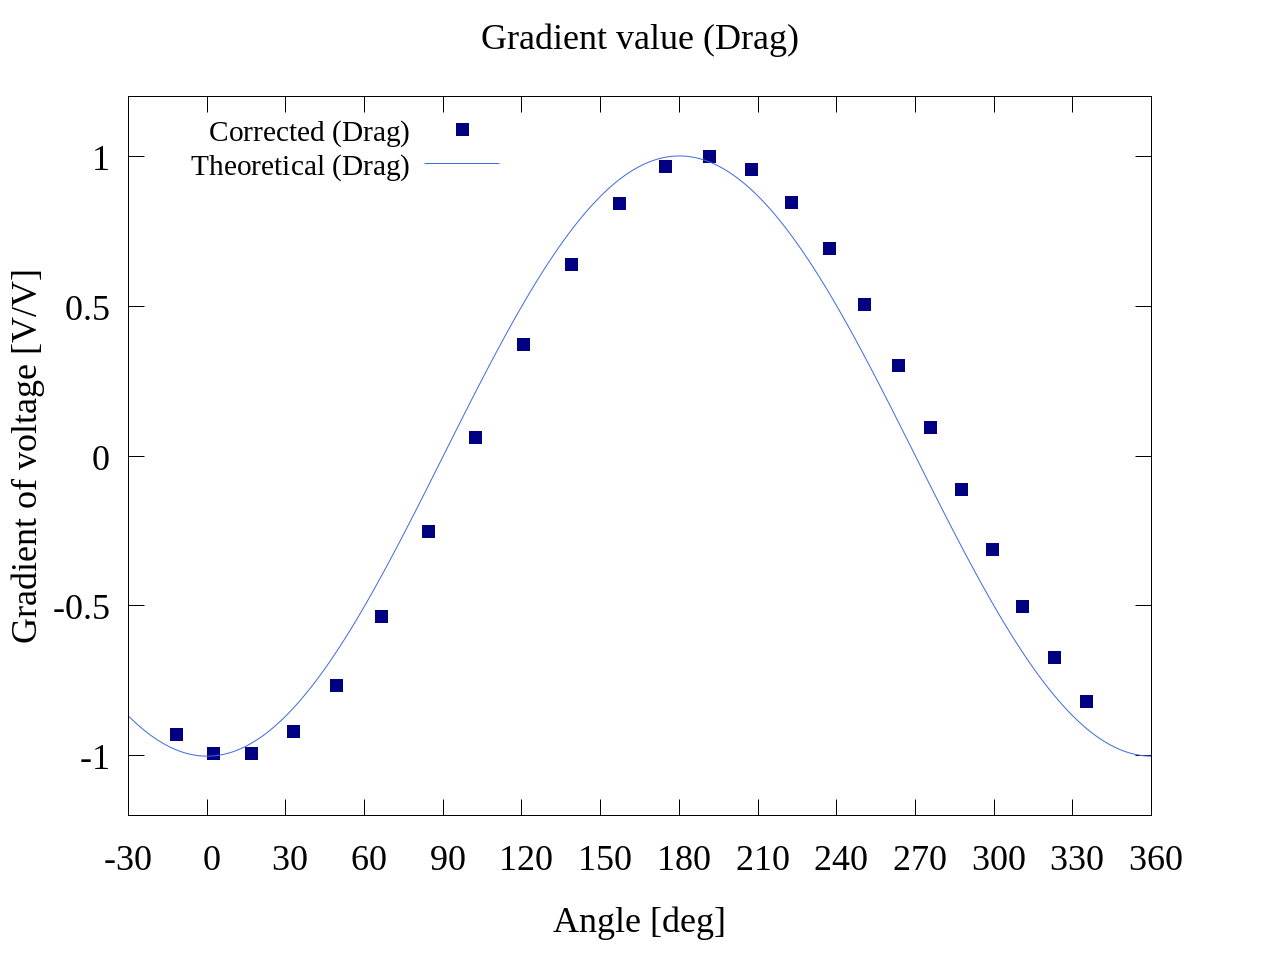
\includegraphics[width=85mm]{../../../02_workspace/result/simulation_tx=10.0_ty=-5.0_dx=5.00_dy=-2.50/plot/21/21-2_corrected_offset_drag.png}
        \caption{Offset corrected value (Drag) }
        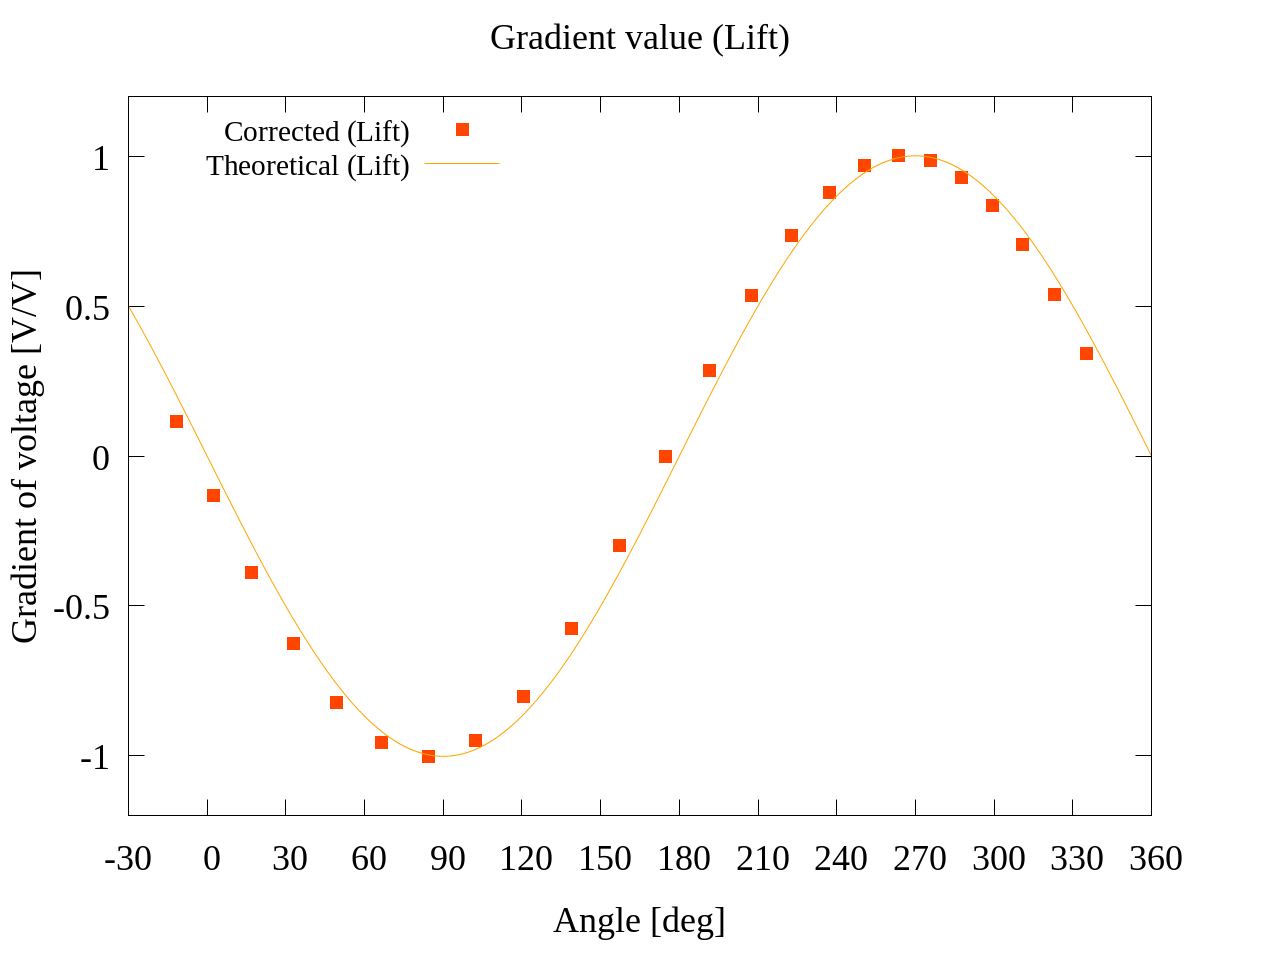
\includegraphics[width=85mm]{../../../02_workspace/result/simulation_tx=10.0_ty=-5.0_dx=5.00_dy=-2.50/plot/21/21-2_corrected_offset_lift.png}
        \caption{Offset corrected value (lift) }
    \end{center}
\end{figure}

\newpage

理論曲線と比較して,波形の再現はされているが,位相差があるようにみえる.
また,プロットされたデータ間隔は異なることもわかる.
このとき,ラグランジュ補間を用いて,等間隔のデータを得るための処理を行う.
なお,データの採用点については上述の処理によって行うこととする.
ラグランジュ補間を行った結果を以下のFig.,Fig.に示す.


\begin{figure}
    \begin{center}
        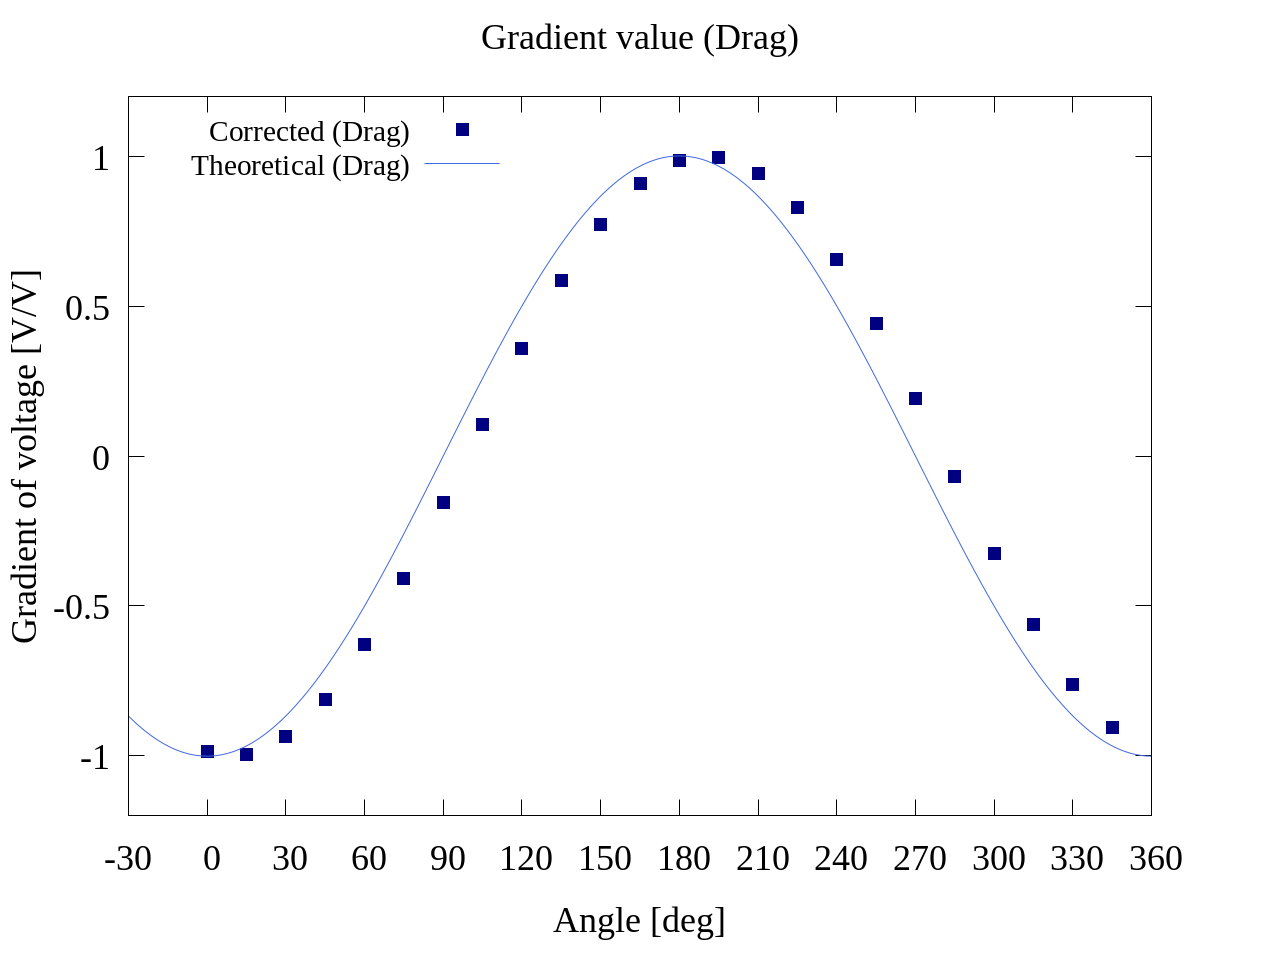
\includegraphics[width=85mm]{../../../02_workspace/result/simulation_tx=10.0_ty=-5.0_dx=5.00_dy=-2.50/plot/21/21-3_interpolated_drag.png}
        \caption{Offset corrected value (Drag) }
        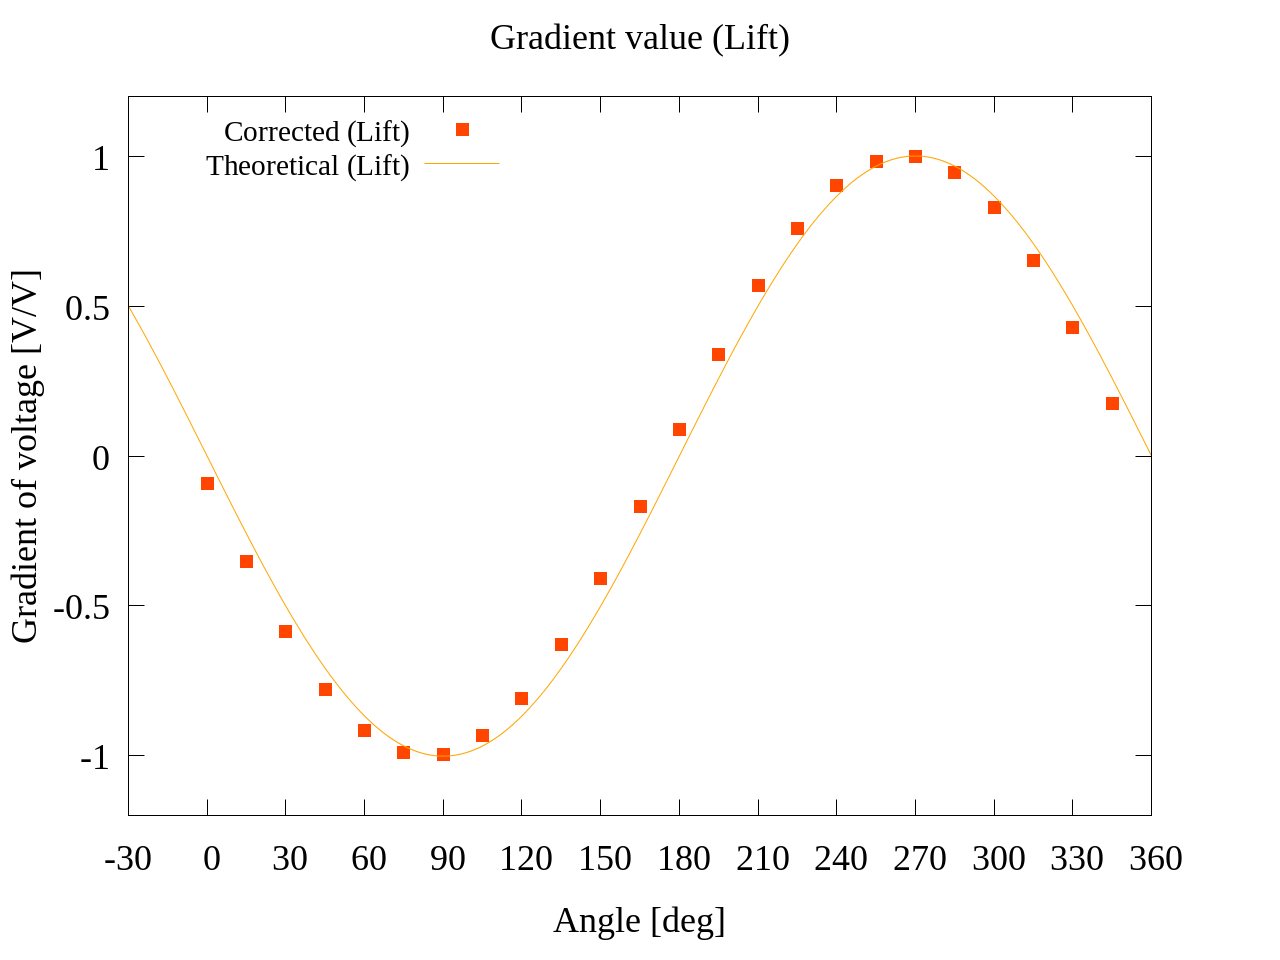
\includegraphics[width=85mm]{../../../02_workspace/result/simulation_tx=10.0_ty=-5.0_dx=5.00_dy=-2.50/plot/21/21-3_interpolated_lift.png}
        \caption{Offset corrected value (lift) }
    \end{center}
\end{figure}


上記のFig.,Fig.と比較すると等間隔のデータを得られていることがわかる.
次に,フーリエ変換を適用する.
このときの結果を以下のFig.,Fig.に示す.
また,波数1の成分についての算出値を以下のTable に示す.

\begin{table}[htbp]
    \begin{center}
        \caption{DFT result value }
        \begin{tabular}{|p{30mm}|p{20mm}|p{20mm}|}
            \hline
            \multicolumn{1}{|c|}{}     & \multicolumn{1}{|c|}{$Re$}    & \multicolumn{1}{|c|}{$Im$}   \\ \hline
            \multicolumn{1}{|c|}{Drag} & \multicolumn{1}{|c|}{-11.835} & \multicolumn{1}{|c|}{2.083}  \\ \hline
            \multicolumn{1}{|c|}{Lift} & \multicolumn{1}{|c|}{-1.081}  & \multicolumn{1}{|c|}{11.978} \\ \hline
        \end{tabular}
    \end{center}
\end{table}

\newpage


\begin{figure}
    \begin{center}
        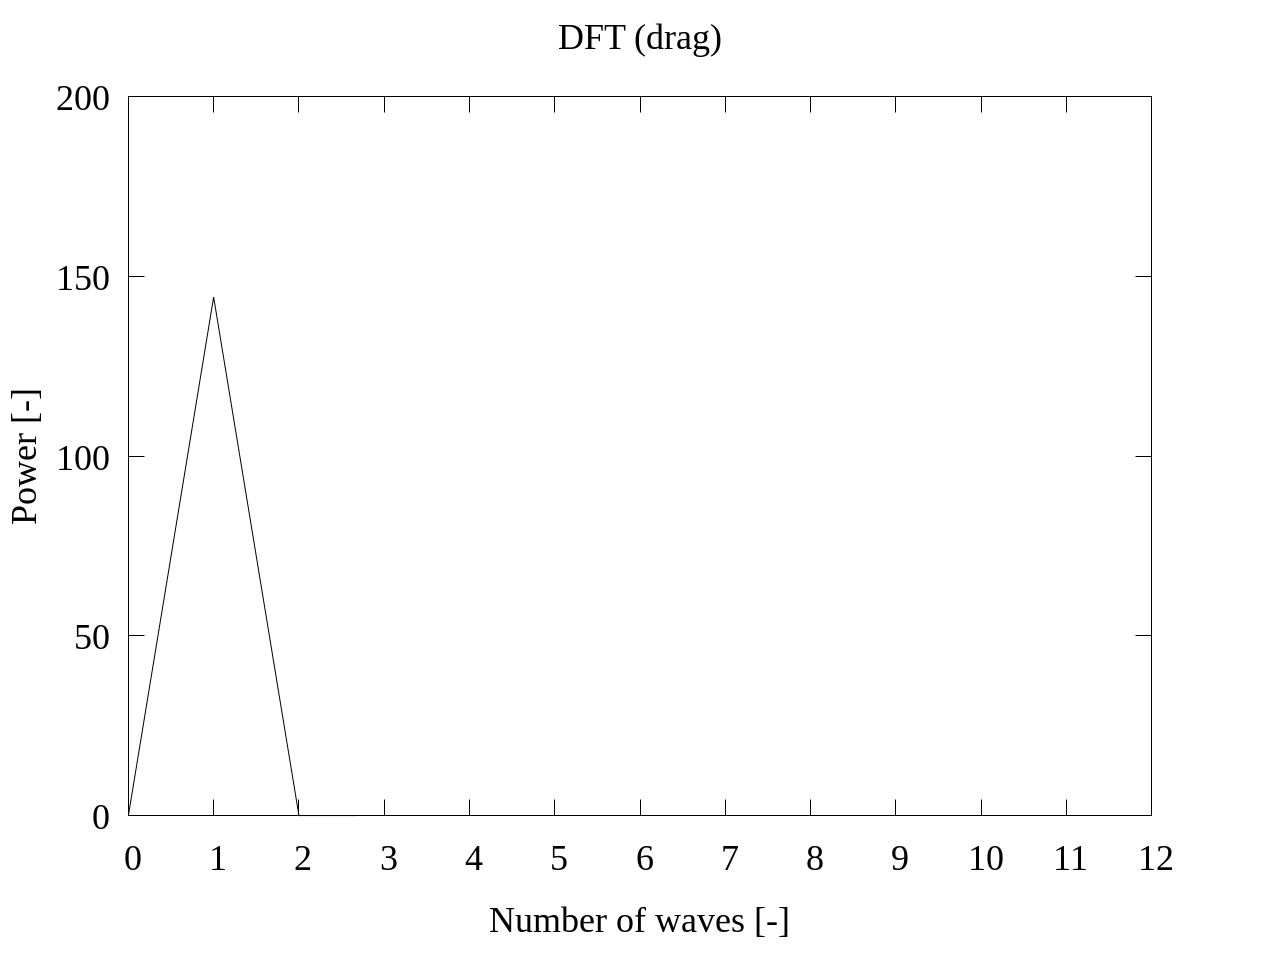
\includegraphics[width=85mm]{../../../02_workspace/result/simulation_tx=10.0_ty=-5.0_dx=5.00_dy=-2.50/plot/07/07-3_dft-drag.png}
        \caption{DFT result (Drag) }
        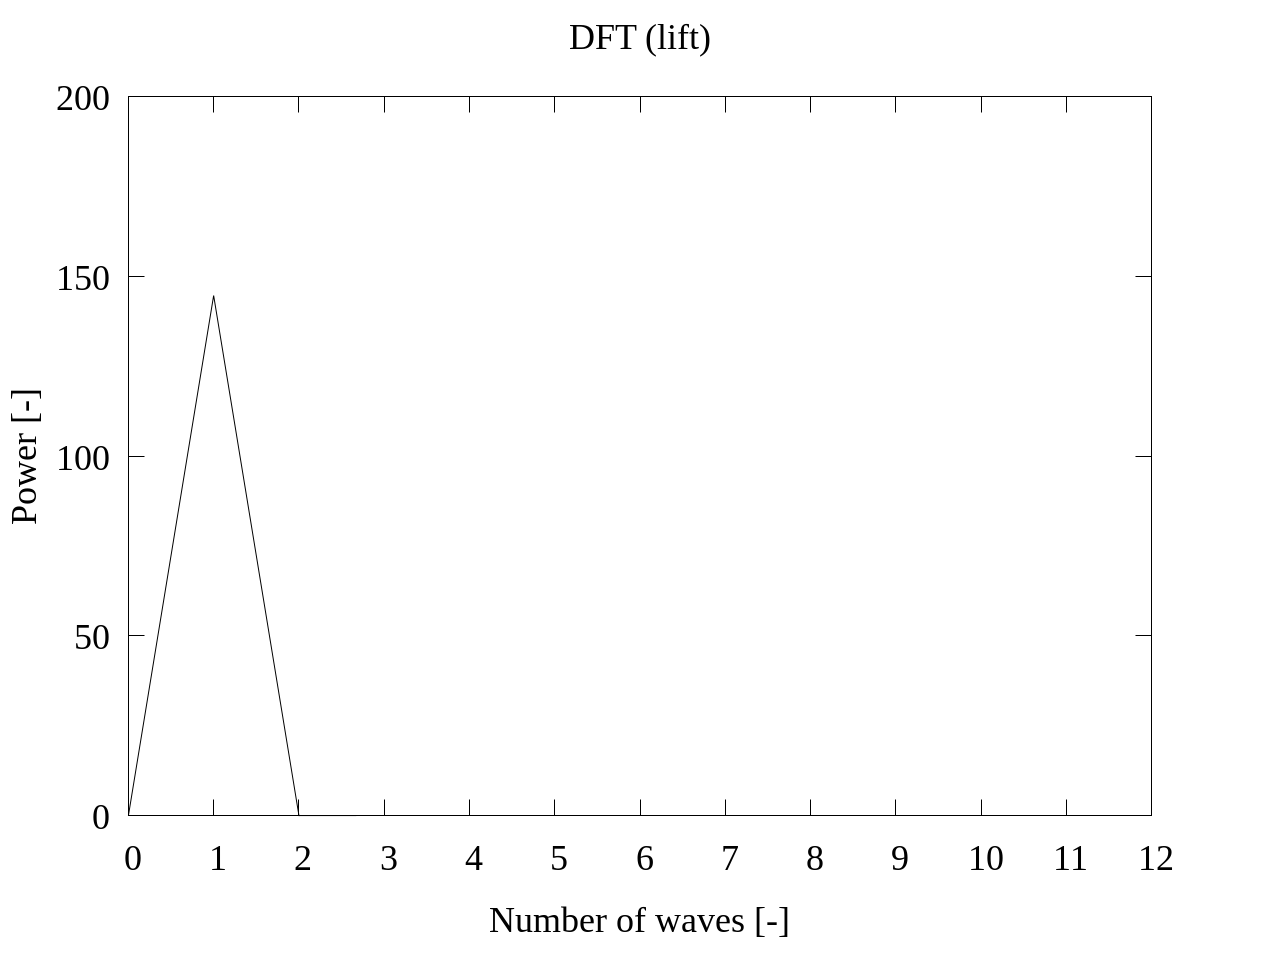
\includegraphics[width=85mm]{../../../02_workspace/result/simulation_tx=10.0_ty=-5.0_dx=5.00_dy=-2.50/plot/07/07-4_dft-lift.png}
        \caption{DFT result (lift) }
    \end{center}
\end{figure}


Fig. ,Fig. より,波数1についてピークがあることがわかり,
座標軸の回転における補正理論の適用結果と同様にデータの特徴を正しく捉えられているといえる.
ここで,Table について,式(),式(),式()より
回転角$\theta_1$,$\theta_2$をそれぞれ算出する.

\begin{table}[htbp]
    \begin{center}
        \caption{Specified rotation angle }
        \begin{tabular}{|p{20mm}|p{20mm}|}
            \hline
            \multicolumn{1}{|c|}{$\theta_1$ [deg]} & \multicolumn{1}{|c|}{$\theta_2$ [deg]} \\ \hline
            \multicolumn{1}{|c|}{10.018}           & \multicolumn{1}{|c|}{-5.158}           \\ \hline
        \end{tabular}
    \end{center}
\end{table}


結果より,算出された回転角$\theta_{1\;\mathrm{test}}$,$\theta_{2\;\mathrm{test}}$は
Table の Case 7 で設定したパラメータと比較すると,異なっていることがわかる.
これは,ラグランジュ補間公式を用いた2次近似による誤差が生じているためと考えられる.

また,算出した回転角$\theta_{1\;\mathrm{test}}$,$\theta_{2\;\mathrm{test}}$を用いて
座標系の回転における補正理論を適用した結果を以下のFig.,Fig.,に示す.

\begin{figure}
    \footnotesize
    \begin{center}
        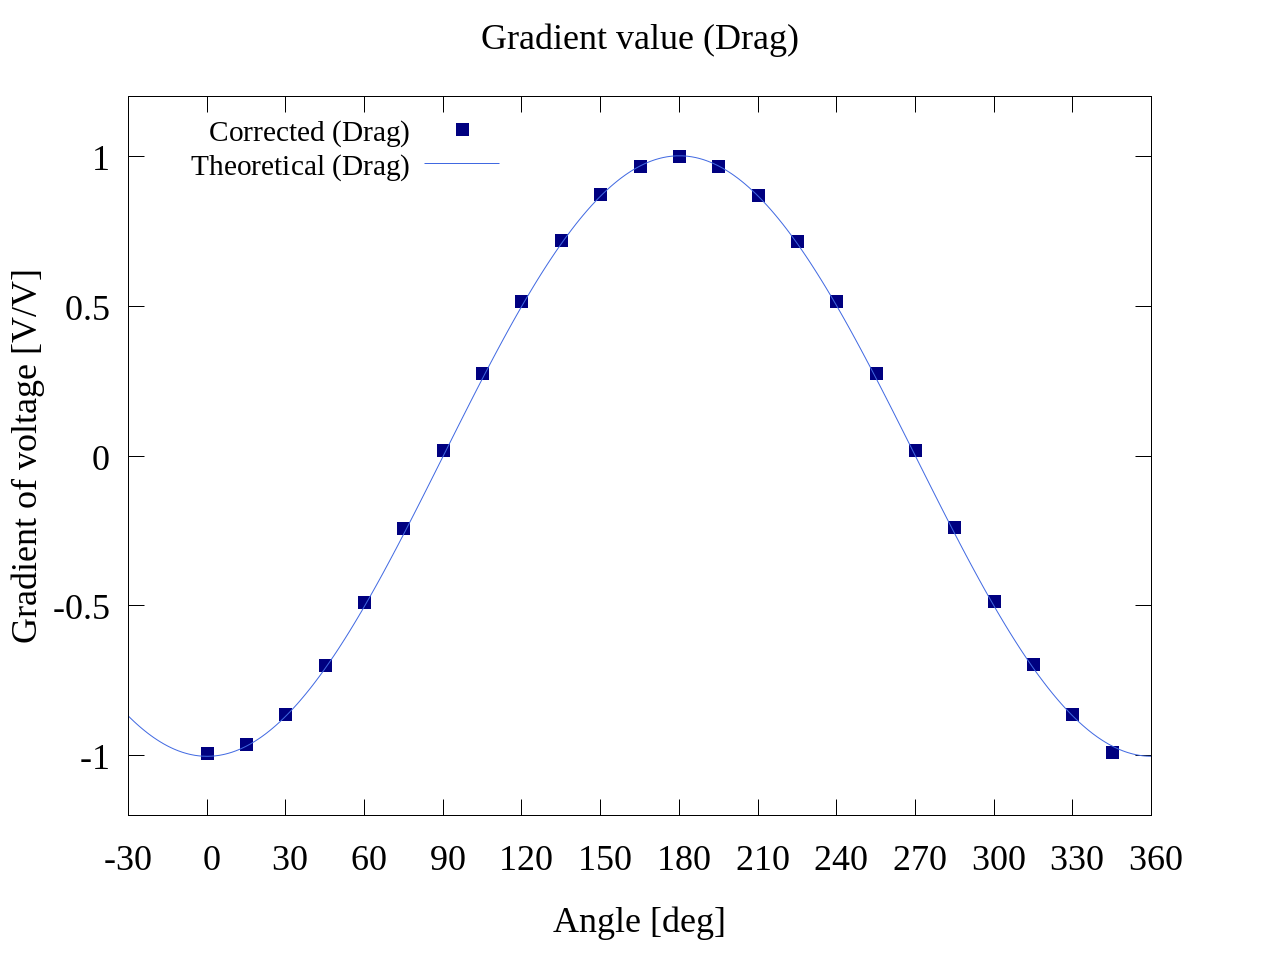
\includegraphics[width=85mm]{../../../02_workspace/result/simulation_tx=10.0_ty=-5.0_dx=5.00_dy=-2.50/plot/21/21-4_corrected_angle_drag.png}
        \caption{Corrected data (Drag) }
        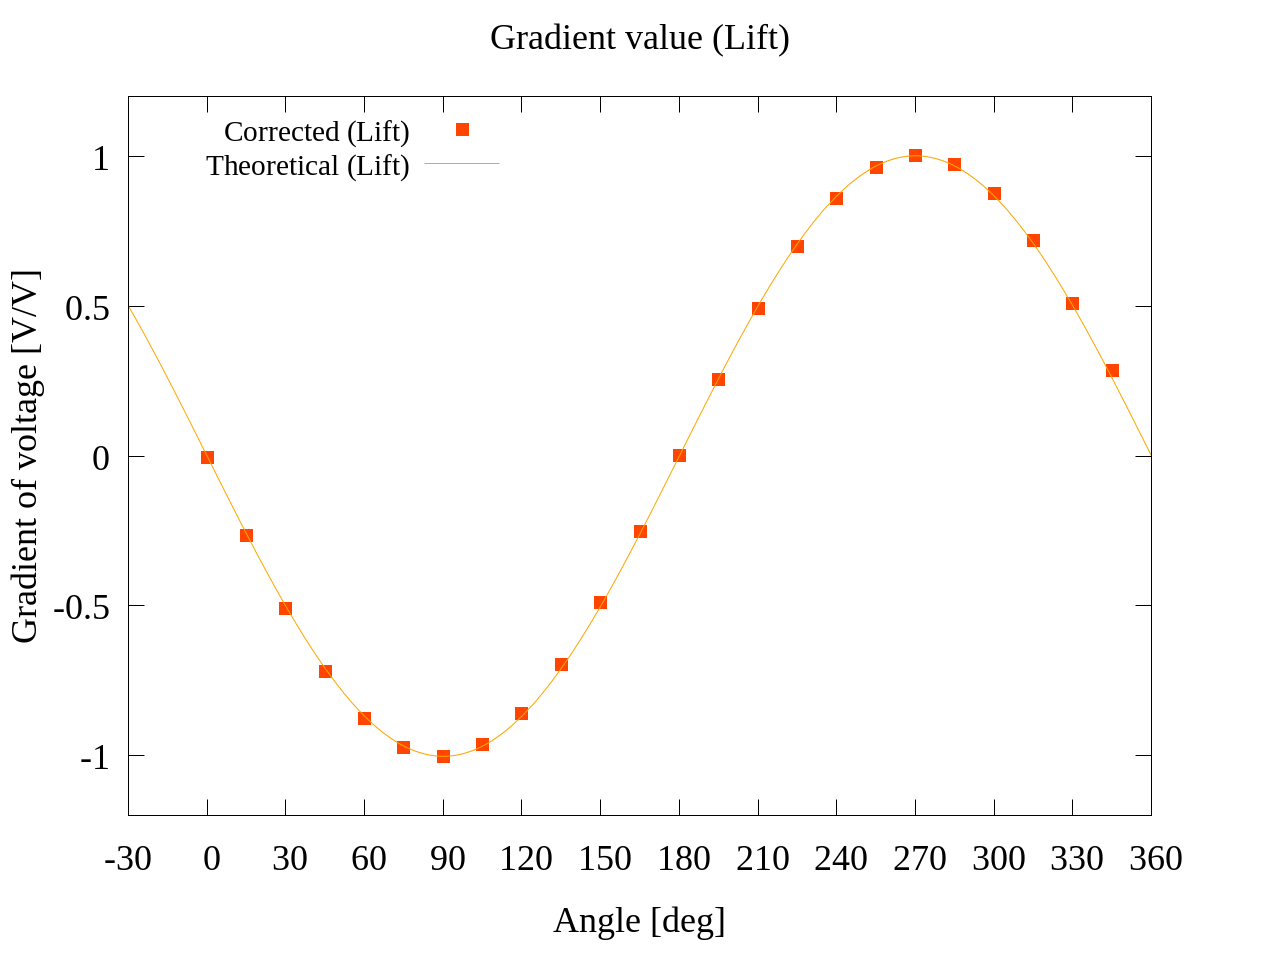
\includegraphics[width=85mm]{../../../02_workspace/result/simulation_tx=10.0_ty=-5.0_dx=5.00_dy=-2.50/plot/21/21-4_corrected_angle_lift.png}
        \caption{Corrected data (Lift) }
    \end{center}
\end{figure}


\section{卒業論文について}

\section{使用する図表}

\end{document}